\documentclass[output=paper]{langsci/langscibook}

\ChapterDOI{10.5281/zenodo.573774}
\title{Beyond binary dependencies in language structure}
\author{Damián E. Blasi\affiliation{University of Zürich, \\Max Planck Institute for the Science of Human History}\lastand Seán G. Roberts\affiliation{Max Planck Institute for Psycholinguistics}
}
\begin{document}
\maketitle

\is{typology} \is{functionalism} \is{cognition} \is{human language faculty} \noindent The study of the regularities in the structures present across languages has always been a quest in close contact with the analysis of data. Traditionally, causal dependencies between pairs of typological variables (like word order patterns or the composition of segment inventories) have been argued for on the basis of language counts, namely how many languages out of a sample exhibit certain patterns in contrast to others. Regularities of this kind have been used in virtually all theoretical camps, and researchers made them part of their discussion on functional pressures on language, cognitive schemes and the architecture of a putative common computational core underlying language, among other things. This popularity resides, without doubt, in the strength and simplicity of the idea: if a set of languages with no recent genealogical history nor traces of areal contact tend to share the same pair of properties again and again, then there seems to be something about the properties of probable languages in general. \is{probable languages}

\is{causality} \is{causal strength} While venerable and potentially useful, this procedure is complicated by many factors.  First, the nature of a proposed dependency can affect how the pattern of observations translates into support for the dependency.  In the first section, we show how different notions of causality and causal strength are appropriate for different types of dependencies involving two variables.  Secondly, these dependencies can be distorted not only by historical relations \is{historical linguistics} between languages (as usually acknowledged in the literature) but also due to complex causal dependencies involving multiple variables.  Addressing these concerns requires appropriate formalisms and statistical techniques. These exist and are widely used for addressing the problem of historical relations \is{historical relations} (which we cover in the second section), but methods for dealing with relationships between more than two variables are underdeveloped in linguistics. In the final section, we discuss some new approaches to detecting causal dependencies between more than two variables.

\section{Probability and causation}
\is{probability} \is{causality} There exist several possible formalizations of the concept of causality inspired in concepts from mathematics, logic, computation and philosophy (see \citealt{fitelson2011probabilistic}). For the kind of regularities and laws governing the language sciences causation appears more naturally described in terms of probabilities. 
 
For the sake of simplicity, we will be dealing in these examples with a hypothesized cause (C) and an effect (E). These will be expressed in terms of total probabilities of the cause or the effect to occur ($P(C)$ and $P(E)$ respectively) and the related conditional probabilities (such as the probability of the effect occurring given that the cause is present $P(E {\mid}  C)$, or the probability of the effect occurring given that the cause is absent $P(E{\mid}{}{\sim}C)$).  In this context, we can think about causation as probability raising: the probability of the effect taking place is larger when the cause is present than when the cause is absent, $P(E{\mid}{}C) > P(E{\mid}{}{\sim}C)$. 

It is critical to remark that these probabilities and the measures of strength are used as a way of thinking about causal relations instead of definitions suitable for statistical analysis. Identifying probabilities with type frequencies and determining causal dependencies by attesting patterns in language counts can be problematic, and as such the structure of the models we use to think about the data and the data themselves (and their statistical properties) should be always clearly distinguished.
 
Typically, probabilities are equated to frequencies of occurrence when the statistical assessment takes place. $P(E)$ is approximated to the proportion of times the cause is observed to occur compared to not occurring, and $P(E{\mid}{}{\sim}C)$ to the proportion of times the effect is observed when the cause is absent. For instance, given the contingency table in \ref{tab:blasi:(1)},
 

\ea \label{tab:blasi:(1)}
%  \begin{table}
\begin{tabular}{rrr}
%  \lsptoprule
 & C & $\sim$ C \\
 \midrule
E & 10 & 5 \\
% \hline
${\sim}$E & 5 & 25 \\
%  \lspbottomrule
\end{tabular}
% \end{table}
\z

\newpage 
\noindent
we could readily estimate $P(C)$=15/45=1/3 and $P(E{\mid}{}{\sim}C)$=5/30=1/5. This is the usual practice in the field, but it hides a number of assumptions about what is tested and the nature of the sampling process.

First of all, the strategy of counting languages has been used sometimes to say something about probable languages in general and not about the particular relations that hold in the necessarily contingent set of surveyed languages. This is as fundamental as it is uncontroversial and pervades scientific practice, and in particular the language sciences -- we infer general properties of cognition \is{cognition} from a limited sample of experimental participants and we determine the usage properties \is{usage properties} of words from samples of text that are diminishingly small in comparison to what is regularly produced by speakers. 

\is{typology} In consequence, we assume that the frequency measured in a given set of typological data matches, in some way, the likelihood of picking at random any likely human language and finding that it has a certain property. This becomes explicit in the linguistic typology literature: in the absence of mechanisms or constraints shaping the structure of the grammar, we ``would expect each type to have roughly an equal number of representatives'' \citep{comrie1989language}. The issue stems from the fact that what ``roughly'' means here is left unspecified and to a large extent at the discretion of the researcher. In fact, any reasonable sampling model \is{sampling models} will generate observable differences in the proportions even when no effect is present \citep{cysouw2010probability}. Specific distributions of typological variables have been motivated observationally \citep{nichols1992linguistic}, based on concrete models inspired by principles of language change \is{language change} (Cysouw 2010) or borrowed directly from the toolkit of machine learning, \is{machine learning} the Dirichlet process \is{Dirichlet process} being a particularly popular choice that is plastic enough as to reflect our lack of certainty \citep{daume2009non,piantadosi2014quantitative}.  
 
Assuming for a moment now that we do have access to the true probabilities of causes and effects and their relation (perhaps via a careful consideration of the observed frequencies), let us consider now the two simplest cases of causal relations between C and E (illustrated in Figure \ref{fig:Cont}). Greenberg's seminal work on implicational typological universals\is{implicational universals} \is{typology} already presented a binary classification of dependencies into which we will tap due to its popularity (\citealt{greenberg1966universals}, see Culbertson, this volume Cristofaro, this volume). 

\begin{figure}[t]
% 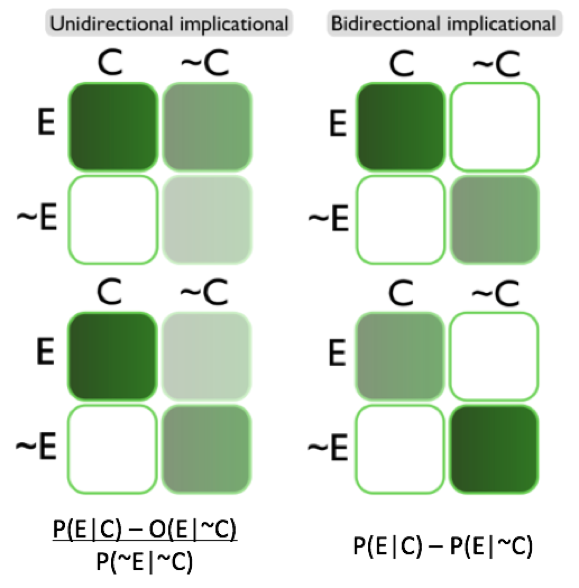
\includegraphics[width=100mm]{figures/blasi-Fig1.png}
% \resizebox{.8\textwidth}{!}{
% \input{figures/Figure1_fixed-BLASI.pdf}}
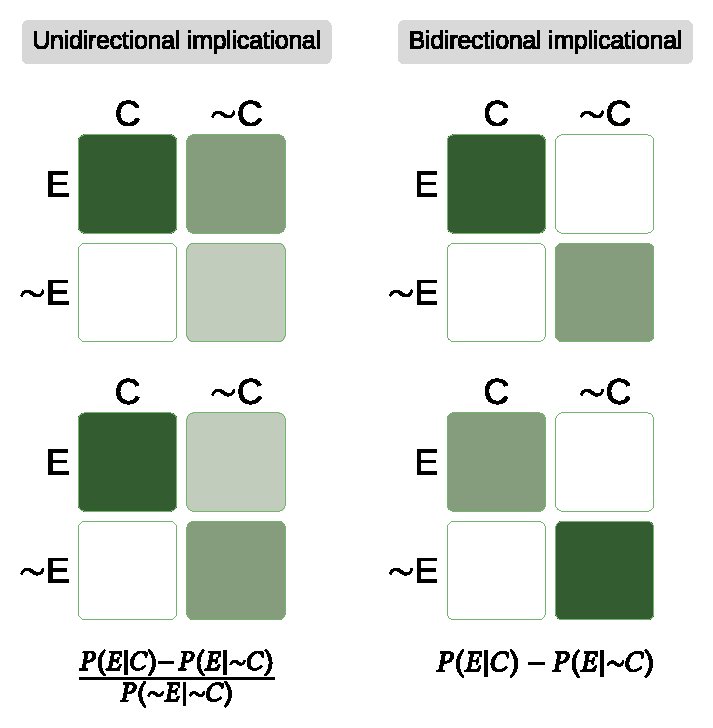
\includegraphics[width=0.8\textwidth]{figures/Figure1_fixed-BLASI.pdf}
\caption{Contingency tables that maximise different measures of causal strength when language type frequencies are equated to type probabilities.  On the left are two tables which maximize unidirectional implications and on the right are two tables which maximize bidirectional implication.  More intense colour stands for more cases attested with those properties; cells in white represent no counts. The formulas for different notions of causal strength appear at the bottom.}
\label{fig:Cont}
\end{figure}
 
\is{implicational universals!bidirectional} \is{implicational universals!unidirectional} \is{implicational universals!bidirectional vs. unidirectional} Some of Greenberg's universals are bidirectional implications, such as the order of adposition and noun implying the order of genitive and noun, and vice versa.  Bidirectional implications contrast with unidirectional implications, which allow the possibility of the effect being present without the cause, but the cause makes the effect more probable. For instance, Greenberg suggested that languages with VSO canonical order tend to be prepositional, though this does not claim that all prepositional languages will be VSO: prepositions occur with virtually all other word order combinations, prominently SVO. \is{prepositional languages} \is{constituent order}

\largerpage
While these ideas are intuitive, the formalization of causal strength by means of probabilities sheds light on the kinds of evidence that are needed in order to put forward any claim about causal influence.  For the sake of convenience, causal measures are often defined in such a way that 1 stands for the strongest causal relation and 0 for the absence of any evidence of a causal effect, with intermediate values reflecting strengths between these extremes. To start with, \cite{eells1991probabilistic}'s view of causal strength captures adequately the causal strength underlying a bidirectional implication, which is defined as:
 
\ea
$CS_e = P(E{\mid}{}C) - P(E{\mid}{}{\sim}C)$
\z

\is{probability} That is, the change in the probability of the effect when the cause is present and when the cause is absent. The largest difference ($CS_e$=1) will be achieved when the cause deterministically triggers the effect ($P(E{\mid}{}C)$=1) and where the absence of the cause also implies the absence of the effect ($P(E{\mid}{}{\sim}C)$=0) -- as represented in Figure \ref{fig:Cont}. On the other hand, when the cause does not change the probability of the effect occurring ($P(E{\mid}{}C)$=$P(E{\mid}{}{\sim}C)$), Eells' measure of causal strength is minimised ($CS_e$=0). Notice that the strength of the assertion of a bidirectional implicational universal does not rely on the relative frequencies of each type, i.e. $P(C)$ and $P(E)$ and their complements. \is{implicational universals!bidirectional}

\is{implicational universals!unidirectional}On the other hand, unidirectional implications do not make any predictions with respect to the case in which the cause is absent. $P(E{\mid}{}{\sim}C)$ could be close to either 1 or 0 without affecting our confidence on the efficacy of the cause -- e.g. that smoking leads convincingly to cancer is independent of the fact that cancer might arise due to other factors as well. However, rather than using the plain conditional probability as a measure of the causal strength of a unidirectional implication ($P(E{\mid}{}C)$) the probability $P(E{\mid}{}{\sim}C)$ plays the role of a baseline to compare against. Thus, a good normalized measure of causal strength for unidirectional implications would be one that (1) becomes 0 when the cause does not make the effect more or less probable than its absence and (2) is 1 only when the cause yields the effect determinstically ($P(E{\mid}{}C)$=1). This leads to none other than \cite{cheng1997covariation}'s notion of causal strength: \is{causal strength} \is{probability}

\ea
$CS_c$ = $\left[P(E{\mid}{}C) - P(E{\mid}{}{\sim}C)\right]$ / $P({\sim}E{\mid}{}{\sim}C)$
\z

That is, the causal power increases as we observe the effect with the cause and decreases as we observe the effect with the cause, but only to the extent that we also observe no effect without the cause.  

\is{causal strength} \is{implicational universals!unidirectional} In contrast to the idea that causality constitutes a monolithic phenomenon, there are many other approaches to the notion of causal strength (see  \citealt{fitelson2011probabilistic}), each one being suitable for the study of different dependencies.   The notion of causal measure will also impact the strategy of inference of the involved probabilities. For example, a unidirectional implication could be assessed by collecting data only on languages which are known to exhibit the cause, while a bidirectional implication requires knowing about languages both with and without the cause. \is{implicational universals!bidirectional}

\section{Moving towards statistical support}

The formalisms above rely on knowing the real probabilities of each cell in the contingency table.  The question of practical interest, then, is how to make a statistically valid case for a dependency based on language counts.  These counts might differ considerably from the true probabilities since simple co-occurrence in a sample of data does not guarantee dependency. The most well-known sources of inflated co-occurrences without substantial causal links are shared history or contact. \is{language contact} For instance, in the Mesoamerican linguistic area, \is{Meso-American languages} languages frequently display a vigesimal numeral system and they lack switch-reference, traits that distinguish them from neighbouring languages \citep{campbell1986meso}. A contingency table displaying the number of languages in that region would give the impression that both variables are associated, which will be simply reflecting the fact that those traits have been transmitted \is{transmission} together all the way down the genealogical tree or horizontally \is{transmission!genealogical} \is{transmission!horizontal} from other language(s). This confound -- known as Galton's problem -- applies to any study trying to detect causal connections between traits in languages.  \cite{roberts2013linguistic} demonstrate how pervasive this problem can be by finding co-occurrences between traits with no causal dependencies between them.  

\is{regression methods} \is{mixed effects model framework} \is{implicational universals!bidirectional} These problems can be overcome if the history of contact between languages is taken into account.  For example, bidirectional implications can be easily captured by the many regression methods available. \citet{jaeger2011mixed} recommend a mixed effects model framework so as to be able to account for areal and genealogical dependencies as random effects for that purpose. Another alternative is to use explicit phylogenetic \is{phylogeny} information and map branch lengths to covariance (so languages that diverged more recently in time are expected to have more similar feature values) \citep{Verkerk2014}. The Family Bias method \is{Family Bias method} \citep{bickel2013distributional} continues the tradition of comparing larger linguistic groupings in a regular regression setting (without any special specification of the covariance between languages) but instead infers the biases of the groupings by assessing the evidence in favour or against one particular typological variant (or set of variants). \is{implicational universals!unidirectional}
The literature on the statistical assessment of unidirectional implications is much less restricted, however. Researchers have devised ways of resolving this issue within the frequentist \citep{Everett2015} and Bayesian traditions \citep{daumecampbell2009}.

Another way that co-occurrence probabilities can be distorted, and one that is rarely addressed, involves more complicated causal dependencies.  The statistical methods mentioned above become limited when more than two variables are taken into account at a time and indeed, perhaps as an implicit acknowledgement of this difficulty, most typological generalizations are limited to pairs of variables rather than more complex constellations. 

Let us see more precisely how complex dependencies might yield spurious dependencies by considering the simplest possible case beyond the two-variable case, which is naturally when there are three variables causally linked in some way. If we regard causal relations graphically as arrows going from the causes to the effects, then this setting will correspond to any of four different possible arrangements depicted in Figure \ref{fig:vars}.


\begin{figure}
% 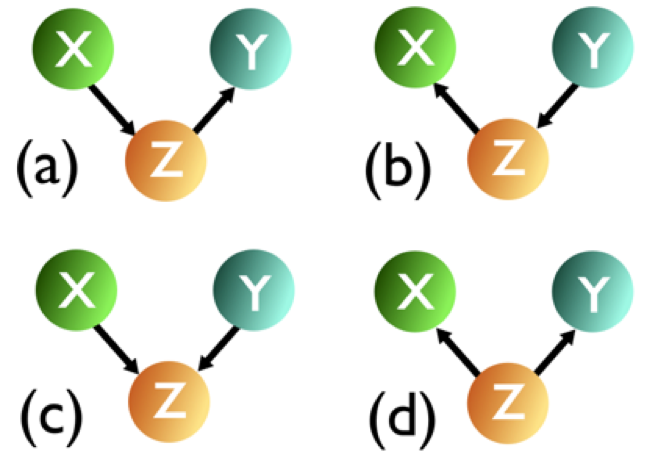
\includegraphics[width=80mm]{figures/blasi-Fig2.png}

\resizebox{.6\textwidth}{!}{
%\documentclass[a4paper,12pt]{article}
%
%\usepackage{color}
%
%\usepackage[cmyk]{xcolor}
%\definecolor{blasi-gold}{cmyk}{0,0.42,0.76,0.18} 
%\definecolor{blasi-turq}{cmyk}{0.39,0,0.09,0.17} 
%\definecolor{blasi-green}{cmyk}{0.43,0,0.64,0.08} 
%
%\usepackage{tikz}
%\usetikzlibrary{positioning}
%
%\pagestyle{empty}
%
%\begin{document}
%	
\begin{tikzpicture}[baseline]
\tikzset{every node/.style={text=white}}

\node at (0,0) (a_z) [fill=blasi-gold, circle, radius=1cm] {\sffamily\bfseries Z};
\node (a_x) [above left=1em and 1em  of a_z, fill=blasi-green, circle, radius=1cm] {\sffamily\bfseries X};
\node (a_y) [above right=1em and 1em  of a_z, fill=blasi-turq, circle, radius=1cm] {\sffamily\bfseries Y};
\node [below=\baselineskip of a_z, text=black] {\sffamily (a)};

\draw [very thick,->] (a_x) -- (a_z); \draw [very thick,->] (a_z) -- (a_y);

\node at (3,0) (b_z) [fill=blasi-gold, circle, radius=1cm] {\sffamily\bfseries Z};
\node (b_x) [above left=1em and 1em  of b_z, fill=blasi-green, circle, radius=1cm] {\sffamily\bfseries X};
\node (b_y) [above right=1em and 1em  of b_z, fill=blasi-turq, circle, radius=1cm] {\sffamily\bfseries Y};
\node [below=\baselineskip of b_z, text=black] {\sffamily (b)};

\draw [very thick,<-] (b_x) -- (b_z); \draw [very thick,<-] (b_z) -- (b_y);

\node at (0,-3) (c_z) [fill=blasi-gold, circle, radius=1cm] {\sffamily\bfseries Z};
\node (c_x) [above left=1em and 1em  of c_z, fill=blasi-green, circle, radius=1cm] {\sffamily\bfseries X};
\node (c_y) [above right=1em and 1em  of c_z, fill=blasi-turq, circle, radius=1cm] {\sffamily\bfseries Y};
\node [below=\baselineskip of c_z, text=black] {\sffamily (c)};

\draw [very thick,->] (c_x) -- (c_z); \draw [very thick,<-] (c_z) -- (c_y);

\node at (3,-3) (d_z) [fill=blasi-gold, circle, radius=1cm] {\sffamily\bfseries Z};
\node (d_x) [above left=1em and 1em  of d_z, fill=blasi-green, circle, radius=1cm] {\sffamily\bfseries X};
\node (d_y) [above right=1em and 1em  of d_z, fill=blasi-turq, circle, radius=1cm] {\sffamily\bfseries Y};
\node [below=\baselineskip of d_z, text=black] {\sffamily (d)};

\draw [very thick,<-] (d_x) -- (d_z); \draw [very thick,->] (d_z) -- (d_y);
\end{tikzpicture}

%\end{document}
}

\caption{Four possible (non-trivial) ways in which variables X, Y and Z could be causally linked.  Arrows represent the flow of causality, so that an arrow pointing from X to Z indicates that changes to X cause changes in Z.}
\label{fig:vars}
\end{figure}


\is{morphological complexity} \is{L2 speakers} The first two cases (a and b in Figure \ref{fig:vars}) correspond to Z simply serving as a communicator of the effect of X on Y or vice versa. For instance, it has been suggested that population size and morphological complexity are causally connected via the number of L2 speakers \citep{lupyan2010language}: the larger the population (X), the more likely it is that the language comes into contact with other languages, increasing the number of L2 speakers (Z) which act upon the language by simplifying the system of its morphological structures (Y).
 
The third possibility is that Z is causing both X and Y (d in Figure \ref{fig:vars}), so the observed causal link between the two is an artifact of Z being a common cause. As an example, many languages of the world have noun classes (X) also have applicative voice (Y) \citep{aronoff2011morphology}. The common cause behind the joint occurrence of these features is that many of these languages come from the \ili{Atlantic-Congo} family (Z), one of the largest linguistic families.
 
\is{isolating languages} Finally, it could be that both X and Y contribute jointly to cause Z (c in Figure \ref{fig:vars}). Languages with isolating morphology (X) will naturally have shorter words in average (Z), and the same is true for languages with tones (Y).
 
\is{implicational universals} The qualitative Greenbergian implications presented before had a transparent formal counterpart and they can be evaluated statistically with well established methods. However, the discussion and evaluation of dependencies involving three or more variables become increasingly unsuitable without a proper formalization. The probabilistic framework discussed at the beginning finds a justification at this point. In addition to it, we need to briefly review some definitions and concepts from graph theory (see \citealt{pearl2009causality}). \is{graph theory}
 
A graph consists of a set of nodes and a set of edges. Directed edges bind two nodes in an asymmetrical fashion -- so if A and B are nodes, either A\textrightarrow B or A\textleftarrow B. A sequence of nodes from A to B where each adjacent pair is bound by a directed edge going from the first to the second member is referred to as a path between A and B. A path that starts and finishes in the same node is referred to as a cycle.  A directed graph is one in which all edges are directed, and a directed graph with no cycles is called a directed acyclic graph (DAG).

The set of nodes that can be reached through a path from A are A's descendants, and the nodes that are directly connected to A such that their common edge points to A (like B\textrightarrow A) are the parents of A.  In DAGs there are no paths which go from a descendant back to one of its parents. 
 
This graphical framework allows a straightforward visualization of causal connections between variables.  Variables are represented as nodes and causal relations (of any kind discussed in the binary case) are represented as directed edges, so A\textrightarrow B will be read as ``A causes B''. The assumption linking this graph representation to the ideas of probabilistic causation discussed before is that of the Markov Causal Condition. \is{Markov Causal Condition} If two variables are dependent and one is not a descendant of the other then their dependency can be explained away by appealing to a common ancestor of the pair.  Put another way, a variable is only affected by its immediately connected (ancestor) causes.
 
\is{Structural equation modelling} Embracing this representation of the relations in the data opens up new statistical possibilities. One that partially relies on regression is to use structural equation models \citep{duncan2014introduction}. Structural equation modelling is a cover term for a number of techniques that allows the testing of more or less well-specified functional dependencies between variables as embedded in DAGs. To take a very basic example (based on a specific case of structural equation modelling called path analysis), suppose that we want to decide between situations (a) and (b) of Figure \ref{fig:vars}. Assuming that we are in possession of good guesses about what could be the functional dependencies, we then could contrast the model fit (how well the model predicts the observed data) between (a) and (b). The possibilities provided by structural equation modelling include the inclusion of hidden variables and non-parametric functional dependencies.
 
In cases where uncertainty about the correct model is high, model comparison might not be the best ally. In those cases, it is possible to appeal to the predictions that come ``for free'' by assuming the Markov Causal Condition along with the DAG. The idea is that the Markov Causal Condition entails a series of conditional dependency statements involving the variables, and that given appropriate conditions it is possible to estimate the most likely underlying causal graph from observational data.  There are multiple methods for doing this \citep{shalizi2013advanced}, a popular efficient and computationally inexpensive method being the PC algorithm \citep{spirtes2000causation,kalisch2012causal}. These techniques are only starting to be explored by researchers in the language sciences \citep{BlasiRobertsMaathuis, Baayen2016}.
 
\section{Conclusion}
The inference of causal dependencies based on surveys of languages has a long history in the field. This methodology faces several complications, like the difficulty of estimating probabilities from counts of languages or the lack of consideration of higher-order dependencies between multiple variables. Methods and formalisms based on probability can address these problems, and help linguists to better test and think about the nature of dependencies in language.

 
\section*{Acknowledgements}
We would like to thank the participants of the Dependencies workshop, and in particular Jennifer Culbertson for helpful feedback.  SR is supported by an ERC Advanced Grant No. 269484 INTERACT to Stephen Levinson. We thank the Max Planck Society for additional support.



{\sloppy
\printbibliography[heading=subbibliography,notkeyword=this]
}

\end{document} 